\intro


\section{О чем идет речь. Основные определения}
% - что такое белки
% - из чего состоят
% - что такое поверхность белка
% - информация о вторичной структуре 
%(мб сказать что такое вторичная структура белка?  вынести во введение или первую главу)

\textbf{Первичная структура} белка задается последовательностью (\textbf{цепочкой}) аминокислот:

\resizebox{\textwidth}{!}{
%\input{aa3_5.tex}
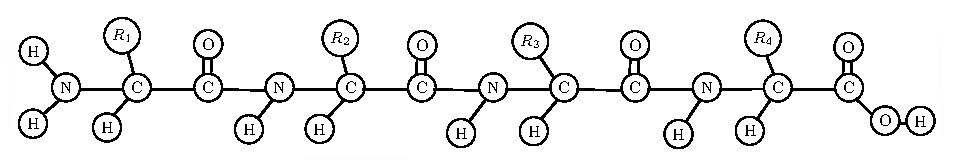
\includegraphics{aa3_1.eps}
}

\textbf{Вторичная структура} задается укладкой цепочки аминокислот в пространственные структуры, \textbf{третичная структура} - расположением этих структур в пространстве в случае, когда белок содержит только одну цепь.

Когда белок состоит из нескольких цепей, говорят о его \textbf{четвертичной структуре}.

\subsection{Белки и энергия}
С точки зрения химии, разным видам структуры соответствуют разные виды химических связей и электростатических взаимодействий.

Когда мы рассматриваем несколько цепочек в составе одного белка или несколько белков, образующих комплекс, мы говорим о \textbf{белок-белковом взаимодействии}.

\textbf{Интерфейс} такого взаимодействия -- это участки \textbf{поверхности} белков, непосредственно контактирующие между собой.



\section{Общие слова}
Диссертация состоит из четырех глав. 
во второй главе приведено описание алгоритма, который используется для выбора регионов

в третьей приведено описание используемой модификации протокола аланинового сканирования, причины использования этого протокола, а также сравнение результатов при выборе регионов по-умолчанию или при выборе регионов разработанным методом 

вспомнить, что я хотела от 4 главы